\section{Flash storage and filesystems}

\begin{frame}
  \frametitle{Block devices vs flash devices: reminder}
  \begin{itemize}
  \item Block devices:
    \begin{itemize}
    \item Allow for random data access using fixed size blocks
    \item Do not require special care when writing on the media
    \item Block size is relatively small (minimum 512 bytes, can be
      increased for performance reasons)
    \item Considered as reliable (if the storage media is not, some
      hardware or software parts are supposed to make it reliable)
    \end{itemize}
  \item Flash devices:
    \begin{itemize}
    \item Allow for random data access too
    \item Require special care before writing on the media (erasing
      the region you are about to write on)
    \item Erase, write and read operation might not use the same block
      size
    \item Reliability depends on the flash technology
    \end{itemize}
  \end{itemize}
\end{frame}

\begin{frame}
  \frametitle{NAND flash chips: how they work ?}
  \begin{itemize}
  \item Encode bits with voltage levels
  \item Start with all bits set to 1
  \item Programming implies changing some bits from 1 to 0
  \item Restoring bits to 1 is done via the ERASE operation
  \item Programming and erasing is not done on a per bit or per byte
    basis
  \item Organization
    \begin{itemize}
    \item Page: minimum unit for PROGRAM operation
    \item Block: minimum unit for ERASE operation
    \end{itemize}
  \end{itemize}
\end{frame}

\begin{frame}{NAND flash storage: organization}
  \begin{center}
    \includegraphics[scale=0.3]{slides/sysdev-flash-filesystems/nand-organization.pdf}
  \end{center}
\end{frame}

\begin{frame}
  \frametitle{NAND flash storage: constraints}
  \begin{itemize}
  \item Reliability
    \begin{itemize}
    \item Far less reliable than NOR flash
    \item Reliability depends on the NAND flash technology (SLC, MLC)
    \item Require additional mechanisms to recover from bit flips: ECC
      (Error Correcting Code)
    \item ECC information stored in the OOB (Out-of-band area)
    \end{itemize}
  \item Lifetime
    \begin{itemize}
    \item Short lifetime compared to other storage media
    \item Lifetime depends on the NAND flash technology (SLC, MLC):
      between 1000000 and 1000 erase cycles per block
    \item Wear leveling mechanisms are required
    \item Bad block detection/handling required too
    \end{itemize}
  \item Despite the number of constraints brought by NAND they are
    widely used in embedded systems for several reasons:
    \begin{itemize}
    \item Cheaper than other flash technologies
    \item Provide high capacity storage
    \item Provide good performance (both in read and write access)
    \end{itemize}
  \end{itemize}
\end{frame}

\begin{frame}
  \frametitle{NAND flash: ECC}
  \begin{itemize}
  \item ECC partly addresses the reliability problem on NAND flash
  \item Operates on blocks (usually 512 or 1024 bytes)
  \item ECC data are stored in the OOB area
  \item Three algorithms:
    \begin{itemize}
    \item Hamming: can fixup a single bit per block
    \item Reed-Solomon: can fixup several bits per block
    \item BCH: can fixup several bits per block
    \end{itemize}
  \item BCH and Reed-Solomon strength depends on the size allocated
    for ECC data, which in turn depends on the OOB size
  \item NAND manufacturers specify the required ECC strength in their
    datasheets: ignoring these requirements might compromise data
    integrity
  \end{itemize}
\end{frame}

\begin{frame}
  \frametitle{The MTD subsystem (1)}
  \begin{itemize}
  \item MTD stands for {\em Memory Technology Devices}
  \item Generic subsystem dealing with all types of storage media that
    are not fitting in the block subsystem
  \item Supported media types: RAM, ROM, NOR flash, NAND flash,
    Dataflash
  \item Independent of the communication interface (drivers available
    for parallel, SPI, direct memory mapping, ...)
  \item Abstract storage media characteristics and provide a simple
    API to access MTD devices
  \item MTD device characteristics exposed to users:
    \begin{itemize}
    \item \code{erasesize}: minimum erase size unit
    \item \code{writesize}: minimum write size unit
    \item \code{oobsize}: extra size to store metadata or ECC data
    \item \code{size}: device size
    \item \code{flags}: information about device type and capabilities
    \end{itemize}
  \item Various kind of MTD "users" in the kernel: file-systems, block
    device emulation layers, user space interfaces...
  \end{itemize}
\end{frame}

\begin{frame}
  \frametitle{The MTD subsystem (2)}
  \begin{center}
    \includegraphics[width=\textwidth]{slides/sysdev-flash-filesystems/mtd-architecture.pdf}
  \end{center}
\end{frame}

\begin{frame}
  \frametitle{MTD partitioning}
  \begin{itemize}
  \item MTD devices are usually partitioned
    \begin{itemize}
    \item It allows to use different areas of the flash for different
      purposes: read-only filesystem, read-write filesystem, backup
      areas, bootloader area, kernel area, etc.
    \end{itemize}
  \item Unlike block devices, which contains their own partition
    table, the partitioning of MTD devices is described externally
    (don't want to put it in a flash sector which could become bad)
    \begin{itemize}
    \item Specified in the board Device Tree
    \item Hard-coded into the kernel code (if no Device Tree)
    \item Specified through the kernel command line
    \end{itemize}
  \item Each partition becomes a separate MTD device
    \begin{itemize}
    \item Different from block device labeling (\code{hda3},
      \code{sda2})
    \item \code{/dev/mtd1} is either the second partition of the first
      flash device, or the first partition of the second flash device
    \item Note that the master MTD device (the device those partitions
      belongs to) is not exposed in \code{/dev}
    \end{itemize}
  \end{itemize}
\end{frame}


\begin{frame}[fragile]
  \frametitle{Linux: definition of MTD partitions}
  \small
  The Device Tree is the standard place to define {\em default} MTD partitions
  for platforms with Device Tree support.\\
  Example from \kfile{arch/arm/boot/dts/omap3-overo-base.dtsi}:
\begin{minted}[fontsize=\scriptsize]{perl}
        nand@0,0 {
                linux,mtd-name= "micron,mt29c4g96maz";
                [...]
                ti,nand-ecc-opt = "bch8"
                [...]
                partition@0 {
                        label = "SPL";
                        reg = <0 0x80000>; /* 512KiB */
                };
                partition@80000 {
                        label = "U-Boot";
                        reg = <0x80000 0x1C0000>; /* 1792KiB */
                };
                partition@1c0000 {
                        label = "Environment";
                        reg = <0x240000 0x40000>; /* 256KiB */
                };
                [...]
\end{minted}
\end{frame}

\begin{frame}
  \frametitle{U-Boot: defining MTD partitions (1)}
  \begin{itemize}
  \item U-Boot also provides a way to define MTD partitions on flash devices
  \item Named partitions are easier to use, and much less error prone than using offsets.
  \item U-Boot partition definitions can also be used by Linux too,
    eliminating the risk of mismatches between Linux and U-Boot. 
  \item Use flash specific commands (detailed soon),
    and pass partition names instead of numerical offsets
  \item Example: \code{nand erase.part <partname>}
  \end{itemize}
\end{frame}

\begin{frame}[fragile]
  \frametitle{U-Boot: defining MTD partitions (2)}
  \begin{itemize}
  \item Example:
  {\tiny
  \begin{verbatim}
setenv mtdids nand0=omap2-nand.0
setenv mtdparts mtdparts=omap2-nand.0:512k(X-Loader)ro,1536k(U-Boot)ro,512k(Env),4m(Kernel),-(RootFS)
  \end{verbatim}
  }
  \item This defines 5 partitions in the \code{omap2-nand.0} device:
    \begin{itemize}
    \item \code{1st stage bootloader} (512 KiB, read-only)
    \item \code{U-Boot} (1536 KiB, read-only)
    \item \code{U-Boot environment} (512 KiB)
    \item \code{Kernel} (4 MiB)
    \item \code{Root filesystem} (Remaining space)
    \end{itemize}
  \item Partition sizes must be multiple of the erase block size.
    You can use sizes in hexadecimal too. Remember the below sizes:
    \code{0x20000} = 128k, \code{0x100000} = 1m, \code{0x1000000} = 16m
  \item \code{ro} lists the partition as read only
  \item \code{-} is used to use all the remaining space.
  \end{itemize}
\end{frame}


\begin{frame}[fragile]
  \frametitle{U-Boot: defining MTD partitions (3)}
  Details about the two environment variables needed by U-Boot:
  \begin{itemize}
  \item \code{mtdids} attaches an {\em mtdid} to a flash device.\\
    \code{setenv mtdids <devid>=<mtdid>[,<devid>=<mtdid>]}
    \begin{itemize}
    \item \code{devid}: {\bf U-Boot} device identifier (from
      \code{nand info} or \code{flinfo})
    \item \code{mtdid}: {\bf Linux} mtd identifier. Displayed
      when booting the Linux kernel:
    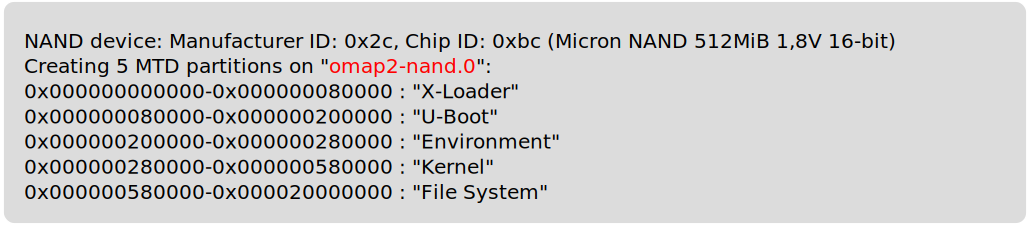
\includegraphics[width=0.85\textwidth]{slides/sysdev-flash-filesystems/kernel-mtd-log.pdf}\\
    \end{itemize}
  \item \code{mtdparts} defines partitions for the different devices\\
  \code{setenv mtdparts mtdparts=<mtdid>:<partition>[,partition]}\\
  \code{partition} format: \code{<size>[@offset](<name>)[ro]}
  \end{itemize}
  Use the \code{mtdparts} command to setup the configuration
  specified by the \code{mtdids} and \code{mtdparts} variables
\end{frame}

\begin{frame}
  \frametitle{U-Boot: sharing partition definitions with Linux}
  Linux understands U-Boot's \code{mtdparts} partition definitions.\\
  Here is a recommended way to pass them from U-Boot to Linux:
  \begin{itemize}
  \item Define a \code{bootargs_base} environment variable:\\
    \code{setenv bootargs_base console=ttyS0 root=....} 
  \item Define the final kernel command line (\code{bootargs})
    through the \code{bootcmd} environment variable:
    \code{setenv bootcmd 'setenv bootargs ${bootargs_base} ${mtdparts};
<rest of bootcmd>'} 
  \end{itemize}
\end{frame}

\begin{frame}
  \frametitle{U-Boot: manipulating NAND devices}
  U-Boot provides a set of commands to manipulate NAND devices,
  grouped under the \code{nand} command
  \begin{itemize}
  \item \code{nand info}\\
    Show available NAND devices and characteristics
  \item \code{nand device [dev]}\\
    Select or display the active NAND device
  \item \code{nand read[.option] <addr> <offset|partname> <size>}\\
    Read data from NAND
  \item \code{nand write[.option] <addr> <offset|partname> <size>}\\
    Write data on NAND
    \begin{itemize}
      \item Use \code{nand write.trimffs} to avoid writing empty pages
      (those filled with \code{0xff})
    \end{itemize}
  \item \code{nand erase <offset> <size>}\\
    Erase a NAND region
  \item \code{nand erase.part <partname>}\\
    Erase a NAND partition
  \item More commands for debugging purposes
  \end{itemize}
\end{frame}

\begin{frame}
  \frametitle{U-Boot: manipulating NOR devices (1)}
  \begin{itemize}
  \item U-Boot provides a set of commands to manipulate NOR devices
  \item Memory mapped NOR devices
    \begin{itemize}
    \item \code{flinfo [devid]}\\
      Display information of all NOR devices
      or a specific one if \code{devid} is provided
    \item \code{cp.[bwl] <src> <target> <count>}\\
      Read/write data from/to the NOR device
    \item \code{erase <start> <end>} or \code{erase <start> +<len>}\\
      Erase a memory region
    \item \code{erase bank <bankid>}\\
      Erase a memory bank
    \item \code{erase all}\\
      Erase all banks
    \item \code{protect on|off <range-description>}\\
      Protect a memory range
    \end{itemize}
  \end{itemize}
\end{frame}

\begin{frame}
  \frametitle{U-Boot: manipulating NOR devices (2)}
  \begin{itemize}
  \item SPI NOR devices
    \begin{itemize}
    \item Grouped under the \code{sf} command
    \item \code{sf probe [[bus:]cs] [hz] [mode]}\\
       Probe a NOR device on
    \item \code{sf read|write <addr> <offset> <len>}\\
       Read/write data from/to a SPI NOR
    \item \code{sf erase <offset> +<len>}\\
       Erase a memory region
    \item \code{sf update <addr> <offset> <len>}\\
       Erase + write operation
    \end{itemize}
  \end{itemize}
\end{frame}

\begin{frame}
  \frametitle{Linux: MTD devices interface with user space}
  \begin{itemize}
  \item MTD devices are visible in \code{/proc/mtd}
  \item The user space only see MTD partitions, not the flash device
    under those partitions
  \item The {\bf mtdchar} driver creates a character device for each
    MTD device/partition of the system
    \begin{itemize}
    \item Usually named \code{/dev/mtdX} or \code{/dev/mtdXro}
    \item Provide \code{ioctl()} to erase and manage the flash
    \item Used by the {\em mtd-utils} utilities
    \end{itemize}
  \end{itemize}
\end{frame}

\begin{frame}
  \frametitle{Linux: user space flash management tools}
  \begin{itemize}
  \item \code{mtd-utils} is a set of utilities to manipulate MTD devices
    \begin{itemize}
    \item \code{mtdinfo} to get detailed information about an MTD device
    \item \code{flash_erase} to partially or completely erase a given
      MTD device
    \item \code{flashcp} to write to NOR flash
    \item \code{nandwrite} to write to NAND flash
    \item Flash filesystem image creation tools: \code{mkfs.jffs2},
      \code{mkfs.ubifs}, \code{ubinize}, etc.
    \end{itemize}
  \item On your workstation: usually available as the \code{mtd-utils}
      package in your distribution.
  \item On your embedded target: most commands now also available
      in BusyBox.
  \item See \url{http://www.linux-mtd.infradead.org/}.
  \end{itemize}
\end{frame}


\begin{frame}
  \frametitle{Flash wear leveling (1)}
  \begin{itemize}
  \item Wear leveling consists in distributing erases over the whole
    flash device to avoid quickly reaching the maximum number of erase
    cycles on blocks that are written really often
  \item Can be done in:
    \begin{itemize}
    \item the filesystem layer (JFFS2, YAFFS2, ...)
    \item an intermediate layer dedicated to wear leveling (UBI)
    \end{itemize}
  \item The wear leveling implementation is what makes your flash
    lifetime good or not
  \end{itemize}
\end{frame}

\begin{frame}
  \frametitle{Flash wear leveling (2)}
  Flash users should also take the limited lifetime of flash
  devices into account by taking additional precautions
  \begin{itemize}
  \item Do not use your flash storage as swap area (rare in embedded
    systems anyway)
  \item Mount your filesystems as read-only, or use read-only
    filesystems (SquashFS), whenever possible.
  \item Keep volatile files in RAM (tmpfs)
  \item Don't use the \code{sync} mount option (commits writes
    immediately). Use the \code{fsync()} system call for per-file
    synchronization.
  \end{itemize}
\end{frame}

\begin{frame}
  \frametitle{Flash file-systems}
  \begin{itemize}
  \item 'Standard' file systems are meant to work on block devices
  \item Specific file systems have been developed to deal flash
    constraints
  \item These file systems are relying on the MTD layer to access
    flash chips
  \item There are several legacy flash filesystems which might be
    useful for specific usage: JFFS2, YAFFS2.
  \item Nowadays, UBI/UBIFS is the de facto standard for medium to
    large capacity NANDs (above 128MB)
  \end{itemize}
\end{frame}

\begin{frame}
  \frametitle{Legacy flash filesystems: JFFS2}
  \begin{columns}
    \column{0.7\textwidth}
    \begin{itemize}
    \item Supports on the fly compression
    \item Wear leveling, power failure resistant
    \item Available in the official Linux kernel
    \item Boot time depends on the filesystem size: doesn't scale well
      for large partitions.
    \item \url{http://www.linux-mtd.infradead.org/doc/jffs2.html}
    \end{itemize}
    \column{0.3\textwidth}
    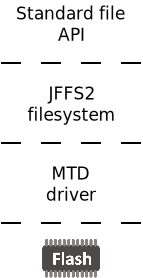
\includegraphics[width=\textwidth]{slides/sysdev-flash-filesystems/jffs2.pdf}
  \end{columns}
\end{frame}

\begin{frame}
  \frametitle{Legacy flash filesystems: YAFFS2}
  \begin{columns}
    \column{0.7\textwidth}
    \begin{itemize}
    \item Mainly supports NAND flash
    \item No compression
    \item Wear leveling, power failure resistant
    \item Fast boot time
    \item Not part of the official Linux kernel: code only available
      separately\\
      (Dual GPL / Proprietary license for non Linux operating systems)
    \item \url{https://yaffs.net/}
    \end{itemize}
    \column{0.3\textwidth}
    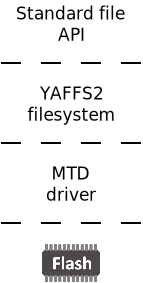
\includegraphics[width=\textwidth]{slides/sysdev-flash-filesystems/yaffs2.pdf}
  \end{columns}
\end{frame}


\begin{frame}
  \frametitle{UBI/UBIFS}
  \begin{columns}
    \column{0.7\textwidth}
    \begin{itemize}
    \item Aimed at replacing JFFS2 by addressing its limitations
    \item Design choices:
      \begin{itemize}
      \item Split the wear leveling and filesystem layers
      \item Add some flexibility
      \item Focus on scalability, performance and reliability
      \end{itemize}
    \item Drawback: introduces noticeable space overhead,
      especially when used on small devices or partitions.
    \end{itemize}
    \column{0.3\textwidth}
    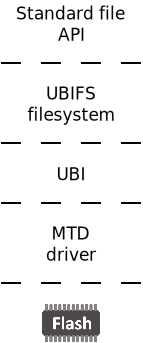
\includegraphics[width=\textwidth]{slides/sysdev-flash-filesystems/ubifs.pdf}
  \end{columns}
\end{frame}

\begin{frame}
  \frametitle{UBI (1)}
  Unsorted Block Images
  \begin{itemize}
  \item \url{http://www.linux-mtd.infradead.org/doc/ubi.html}
  \item Volume management system on top of MTD devices (similar to
    what LVM provides for block devices)
  \item Allows to create multiple logical volumes and spread writes
    across all physical blocks
  \item Takes care of managing the erase blocks and wear
    leveling. Makes filesystems easier to implement
  \item Wear leveling can operate on the whole storage,
    not only on individual partitions (strong advantage)
  \item Volumes can be dynamically resized or, on the opposite, can be
    read-only (static)
  \end{itemize}
\end{frame}

\begin{frame}
  \frametitle{UBI (2)}
  \begin{center}
    \includegraphics[width=\textwidth]{slides/sysdev-flash-filesystems/ubi.pdf}
  \end{center}
\end{frame}

\begin{frame}
  \frametitle{UBI: internals}
  \begin{columns}
    \column{0.5\textwidth}
    \begin{itemize}
    \item UBI is storing its metadata in-band
    \item In each MTD erase block
    \begin{itemize}
      \item One page is reserved to count the number of erase cycles
      \item Another page is reserved to attach the erase block to a
        UBI volume
      \item The remaining pages are used to store payload data
      \end{itemize}
    \item If the device supports subpage write, the EC and VID headers
      can be stored on the same page
    \end{itemize}
    \column{0.5\textwidth}
    \includegraphics[scale=0.3]{slides/sysdev-flash-filesystems/ubi-leb.pdf}
  \end{columns}
\end{frame}

\begin{frame}
  \frametitle{UBI: good practice}
  \begin{itemize}
  \item UBI is responsible for distributing writes all over the flash
    device: the more space you assign to a partition attached to the
    UBI layer the more efficient the wear leveling will be
  \item If you need partitioning, use UBI volumes not MTD partitions
  \item Some partitions will still have to be MTD partitions: e.g. the
    bootloaders and bootloader environments
  \item If you need extra MTD partitions, try to group them at the end
    or the beginning of the flash device
  \end{itemize}
\end{frame}

\begin{frame}
  \frametitle{UBI layout: bad example}
  \begin{center}
    \includegraphics[width=\textwidth]{slides/sysdev-flash-filesystems/ubifs-bad-layout.pdf}
  \end{center}
\end{frame}

\begin{frame}
  \frametitle{UBI layout: good example}
  \begin{center}
    \includegraphics[width=\textwidth]{slides/sysdev-flash-filesystems/ubifs-good-layout.pdf}
  \end{center}
\end{frame}

\begin{frame}
  \frametitle{UBIFS}
  Unsorted Block Images File System
  \begin{itemize}
  \item \url{http://www.linux-mtd.infradead.org/doc/ubifs.html}
  \item The filesystem part of the UBI/UBIFS couple
  \item Works on top of UBI volumes
  \item Journaling file system providing better performance than
    JFFS2 and addressing its scalability issues
  \item See this paper for more technical details about UBIFS internals
    \url{http://www.linux-mtd.infradead.org/doc/ubifs_whitepaper.pdf}
  \end{itemize}
\end{frame}

\begin{frame}
  \frametitle{Linux: UBI host tools}
  \begin{itemize}
  \item \code{ubinize} is the only host tool for the UBI layer
  \item Creates a UBI image to be flashed on an MTD partition
  \item Takes the following arguments:
    \begin{itemize}
    \item \code{-o <output-file-path>}\\
	Path to the output image file
    \item \code{-p <peb-size>}\\
	The PEB size (MTD erase block size)
    \item \code{-m <min-io-size>}\\
	The minimum write unit size (e.g. MTD write size)
    \item \code{-s <subpage-size>}\\
	Subpage size, only needed if both your flash and your
	flash controller are supporting subpage writes
    \item The last argument is a path to a UBI image description file
	  (see next page for an example)
    \end{itemize}
  \item Example: \code{ubinize -o ubi.img -p 16KiB -m 512 -s 256 ubinize.cfg}
  \end{itemize}
\end{frame}

\begin{frame}[fragile]
  \frametitle{ubinize configuration file}
  \begin{itemize}
  \item Can contain several sections
  \item Each section is describing a UBI volume
  \item \code{static} volumes are meant to store {\bf read-only} blobs of data,
	and get the minimum corresponding size. CRC checks are done on
        them.
  \item A read-only UBIFS filesystem can go in a \code{static}
	volume, but in this case \code{dynamic} volumes are best
        for performance (CRC checking also done at UBIFS level).
  \end{itemize}
  \begin{columns}
    \column{0.33\textwidth}
\small
\begin{verbatim}
[kernel-volume]
mode=ubi
image=zImage
vol_id=1
vol_type=static
vol_name=kernel
\end{verbatim}
    \column{0.33\textwidth}
\small
\begin{verbatim}
[rootfs-volume]
mode=ubi
image=rootfs.ubifs
vol_id=2
vol_size=2MiB
vol_type=dynamic
vol_name=rootfs
\end{verbatim}
    \column{0.33\textwidth}
\small
\begin{verbatim}
[data-volume]
mode=ubi
image=data.ubifs
vol_id=3
vol_size=30MiB
vol_type=dynamic
vol_name=data
vol_flags=autoresize
\end{verbatim}
  \end{columns}
\end{frame}

\begin{frame}
  \frametitle{U-Boot: UBI tools}
  Grouped under the \code{ubi} command
    \begin{itemize}
    \item \code{ubi part <part-name>}\\
	Attach an MTD partition to the UBI layer
    \item \code{ubi info [layout]}\\
	Display UBI device information\\
	(or volume information if the \code{layout} string is passed)
    \item \code{ubi check <vol-name>}\\
	Check if a volume exists
    \item \code{ubi readvol <dest-addr> <vol-name> [<size>]}\\
	Read volume contents
    \item U-Boot also provides tools to update the UBI device contents
    \item Using them is highly discouraged (the U-Boot UBI implementation
      is not entirely stable, and using commands that do not touch the UBI
      metadata is safer)
      \begin{itemize}
      \item \code{ubi createvol <vol-name> [<size>] [<type>]}
      \item \code{ubi removevol <vol-name>}
      \item \code{ubi writevol <src-addr> <vol-name> <size>}
      \end{itemize}
    \end{itemize}
\end{frame}

\begin{frame}
  \frametitle{Linux: UBI target tools (1)}
  \begin{itemize}
  \item Tools used on the target to dynamically create and modify
      UBI elements
  \item UBI device management:
    \begin{itemize}
    \item \code{ubiformat <MTD-device-id>}\\
	Format an MTD partition and preserve Erase Counter information if any
    \item \code{ubiattach -m <MTD-device-id> /dev/ubi_ctrl}\\
	Attach an MTD partition/device to the UBI layer, and create a UBI device
    \item \code{ubidetach -m <MTD-device-id> /dev/ubi_ctrl}\\
	Detach an MTD partition/device from the UBI layer, and remove
        the associated UBI device
    \end{itemize}
  \end{itemize}
\end{frame}

\begin{frame}
  \frametitle{Linux: UBI target tools (2)}
  UBI volume management:
    \begin{itemize}
    \item {\small \code{ubimkvol /dev/ubi<UBI-device-id> -N <name> -s <size>}}\\
	Create a new volume. Use \code{-m} in place of \code{-s <size>}
	if you want to assign all the remaining space to this volume.
    \item {\small \code{ubirmvol /dev/ubi<UBI-device-id> -N <name>}}\\
	Delete a UBI volume
    \item {\small \code{ubiupdatevol /dev/ubi<UBI-device-id>_<UBI-vol-id> [-s <size>] <vol-image-file>}}\\
	Update volume contents
    \item {\small \code{ubirsvol /dev/ubi<UBI-device-id> -N <name> -s <size>}}\\
      	Resize a UBI volume
    \item {\small \code{ubirename /dev/ubi<UBI-device-id>_<UBI-vol-id> <old-name> <new-size>}}\\
	Rename a UBI volume
    \end{itemize}
\end{frame}

\begin{frame}
  \frametitle{Linux tools: BusyBox UBI limitations}
  Beware that the implementation of UBI commands in BusyBox is still
  incomplete. For example:
  \begin{itemize}
    \item \code{ubirsvol} doesn't support \code{-N <name>}. You have
      to use specify the volume to resize by its id (\code{-n num}):\\
      \code{ubirsvol /dev/ubi0 -n 4 -s 64 MiB}
    \item Same constraint for \code{ubirmvol}:\\
      \code{ubirmvol /dev/ubi0 -n 4}
    \end{itemize}
\end{frame} 

\begin{frame}
  \frametitle{Linux: UBIFS host tools}
  UBIFS filesystems images can be created using \code{mkfs.ubifs}
    \begin{itemize}
    \item \code{mkfs.ubifs -m 4096 -e 258048 -c 1000 -r rootfs/ ubifs.img}
      \begin{itemize}
      \item \code{-m 4096}, minimal I/O size\\
                 (see \code{/sys/class/mtd/mtdx/writesize}).
      \item \code{-e 258048}, logical erase block size (smaller than
                 PEB size, can be found in the kernel log after running
 		 \code{ubiattach})
      \item \code{-c 1000}, maximum size of the UBI volume the image
        will be flashed into, in number of logical erase blocks.
        Do not make this number unnecessary big, otherwise the UBIFS
        data structures will be bigger than needed and performance
        will be degraded. Details:
        {\scriptsize\url{http://linux-mtd.infradead.org/faq/ubifs.html\#L_max_leb_cnt}}
      \end{itemize}
    \item Once created
      \begin{itemize}
      \item Can be written to a UBI volume from the target using
        \code{ubiupdatevol}
      \item Or, can be included in a UBI image (using \code{ubinize}
        on the host)
      \end{itemize}
    \end{itemize}
\end{frame}

\begin{frame}
  \frametitle{Linux: UBIFS target tools}
  \begin{itemize}
  \item No specific tools are required to manipulate a UBIFS filesystem
  \item Mounting a UBIFS filesystem is done with \code{mount}:\\
    \code{mount -t ubifs <ubi-device-id>:<volume-name> <mount-point>}
  \item Example:\\
    \code{mount -t ubifs ubi0:data /data}
  \end{itemize}
\end{frame}

\begin{frame}
  \frametitle{Linux: UBI image creation workflow}
  \begin{center}
    \includegraphics[scale=0.3]{slides/sysdev-flash-filesystems/ubi-creation-workflow.pdf}
  \end{center}
\end{frame}

\begin{frame}
  \frametitle{Linux: Using a UBIFS filesystem as root filesystem}
  \begin{itemize}
  \item You just have to pass the following information on the kernel
    command line:
    \begin{itemize}
    \item \code{ubi.mtd=1}\\
      Attach \code{/dev/mtd1} to the UBI layer and create \code{ubi0}
    \item \code{rootfstype=ubifs root=ubi0:rootfs}\\
      Mount the \code{rootfs} volume on ubi0 as a UBIFS filesystem
    \end{itemize}
  \item Example: \code{rootfstype=ubifs ubi.mtd=1 root=ubi0:rootfs}
  \end{itemize}
\end{frame}

\begin{frame}
  \frametitle{Summary: how to boot on a UBIFS filesystem}
  In U-Boot:
  \begin{itemize}
  \item Define partitions:\\
     \code{setenv mtdids ...}\\
     \code{setenv mtdparts ...}\\
  \item Define the base Linux kernel bootargs, specifying booting
     on UBIFS, the UBI volume used as root filesystem, and the MTD
     partition attached to UBI. Example:\\
     \code{setenv bootargs_base console=ttyS0 rootfstype=ubifs
root=ubi0:rootfs ubi.mtd=2 ...}
  \item Define the boot command sequence, loading the U-Boot partition
     definitions, loading kernel and DTB images from UBI partitions,
     and adding \code{mtdparts} to the kernel command
     line. Example:\\
     \code{setenv bootcmd 'mtdparts; ubi part UBI; ubi readvol
0x81000000 kernel; ubi readvol 0x82000000 dtb; setenv bootargs
${bootargs_base} ${mtdparts}; bootz 0x81000000 - 0x82000000'}
  \end{itemize}
\end{frame}

\begin{frame}
  \frametitle{Linux: Block emulation layers}
  \begin{itemize}
  \item Sometimes we need block devices to re-use existing block
    filesystems, especially read-only ones like SquashFs
  \item Linux provides two block emulation layers:
    \begin{itemize}
    \item \code{mtdblock}: block devices emulated on top of MTD devices
    \item \code{ubiblock}: block devices emulated on top of UBI volumes
    \end{itemize}
  \end{itemize}
\end{frame}

\begin{frame}
  \frametitle{Linux: mtdblock}
  \begin{itemize}
  \item The \code{mtdblock} layer creates a block device for each MTD
    device of the system
  \item Usually named \code{/dev/mtdblockX}.
  \item Allows read/write block-level access. However bad blocks are not
    handled, and no wear leveling is done for writes.
  \item For historical reasons, JFFS2 and YAFFS2 filesystems require a
    block device for the \code{mount} command.
  \item {\bf Do not write on \code{mtdblock} devices}
  \end{itemize}
\end{frame}

\begin{frame}
  \frametitle{Linux: ubiblock}
  \begin{itemize}
  \item Implemented by Ezequiel Garcia from Free Electrons.
  \item Preferred over \code{mtdblock} if UBI is available (UBI accounts
    for data retention and wear leveling issues, while MTD does not)
  \item The \code{ubiblock} layer creates {\bf read-only} block devices
    on demand
  \item The user specifies which static volumes (s)he would like to attach
    to \code{ubiblock}
    \begin{itemize}
    \item Through the kernel command line: by passing
      \code{ubi.block=<ubi-dev-id>,<volume-name>}
    \item Using the \code{ubiblock} utility provided by \code{mtd-utils}:
      \code{ubiblock --create <ubi-volume-dev-file>}
    \end{itemize}
   \item Usually named \code{/dev/ubiblockX_Y}, where X is the UBI device
     id and Y is the UBI volume id
  \end{itemize}
\end{frame}

\begin{frame}
  \frametitle{Useful reading}
  \begin{itemize}
  \item Managing flash storage with Linux:\\
    \url{http://free-electrons.com/blog/managing-flash-storage-with-linux/}
  \item Documentation on the linux-mtd website:\\
    \url{http://www.linux-mtd.infradead.org/}
  \item Details about creating UBI and UBIFS images:\\
    \url{http://free-electrons.com/blog/creating-flashing-ubi-ubifs-images/}
  \end{itemize}
\end{frame}

\setuplabframe
{Flash Filesystems}
{
  \begin{itemize}
  \item Creating partitions in your internal flash storage
  \item Creating a UBI image with several volumes and flashing it from
    U-Boot
  \item Manipulating UBI volumes from Linux
  \end{itemize}
}
